\documentclass[aspectratio=43]{beamer}

%\documentclass[handout]{beamer}
%% To make 4 per page
%\usepackage{pgfpages}
%\mode<handout>{\setbeamercolor{background canvas}{bg=white}}
%\pgfpagesuselayout{4 on 1}[letterpaper,landscape]%,border shrink=5mm]

\usetheme{default}
% Slide setup, colour independent

\usepackage{amsmath,amssymb,amsthm}
\usepackage{colortbl}
\usepackage{bm}
\usepackage{xcolor}
\usepackage{dsfont}
\usepackage{setspace}
%\usepackage{subfigure}


% Fields and the like
\def\IC{\mathbb{C}}
\def\IF{\mathbb{F}}
\def\II{\mathbb{I}}
\def\IJ{\mathbb{J}}
\def\IM{\mathbb{M}}
\def\IN{\mathbb{N}}
\def\IP{\mathbb{P}}
\def\IR{\mathbb{R}}
\def\IZ{\mathbb{Z}}
\def\11{\mathds{1}}


% Bold lowercase
\def\ba{\mathbf{a}}
\def\bb{\mathbf{b}}
\def\bc{\mathbf{c}}
\def\bd{\mathbf{d}}
\def\be{\mathbf{e}}
\def\bf{\mathbf{f}}
\def\bh{\mathbf{h}}
\def\bi{\mathbf{i}}
\def\bj{\mathbf{j}}
\def\bk{\mathbf{k}}
\def\bn{\mathbf{n}}
\def\bp{\mathbf{p}}
\def\br{\mathbf{r}}
\def\bs{\mathbf{s}}
\def\bu{\mathbf{u}}
\def\bv{\mathbf{v}}
\def\bw{\mathbf{w}}
\def\bx{\mathbf{x}}
\def\by{\mathbf{y}}
\def\bz{\mathbf{z}}

% Bold capitals
\def\bB{\mathbf{B}}
\def\bD{\mathbf{D}}
\def\bF{\mathbf{F}}
\def\bG{\mathbf{G}}
\def\bI{\mathbf{I}}
\def\bL{\mathbf{L}}
\def\bN{\mathbf{N}}
\def\bP{\mathbf{P}}
\def\bR{\mathbf{R}}
\def\bS{\mathbf{S}}
\def\bT{\mathbf{T}}
\def\bX{\mathbf{X}}

% Bold numbers
\def\b0{\mathbf{0}}

% Bold greek
\bmdefine{\bmu}{\bm{\mu}}
\def\bphi{\bm{\phi}}
\def\bvarphi{\bm{\varphi}}

% Bold red sentence
\def\boldred#1{{\color{red}\textbf{#1}}}
\def\defword#1{{\color{orange}\textbf{#1}}}

% Caligraphic letters
\def\A{\mathcal{A}}
\def\B{\mathcal{B}}
\def\C{\mathcal{C}}
\def\D{\mathcal{D}}
\def\E{\mathcal{E}}
\def\F{\mathcal{F}}
\def\G{\mathcal{G}}
\def\H{\mathcal{H}}
\def\I{\mathcal{I}}
\def\L{\mathcal{L}}
\def\M{\mathcal{M}}
\def\N{\mathcal{N}}
\def\P{\mathcal{P}}
\def\R{\mathcal{R}}
\def\S{\mathcal{S}}
\def\T{\mathcal{T}}
\def\U{\mathcal{U}}
\def\V{\mathcal{V}}

% tt font for code
\def\code#1{{\tt #1}}

% Operators and special symbols
\def\nbOne{{\mathchoice {\rm 1\mskip-4mu l} {\rm 1\mskip-4mu l}
{\rm 1\mskip-4.5mu l} {\rm 1\mskip-5mu l}}}
\def\cov{\ensuremath{\mathsf{cov}}}
\def\Var{\ensuremath{\mathsf{Var}\ }}
\def\Im{\textrm{Im}\;}
\def\Re{\textrm{Re}\;}
\def\det{\ensuremath{\mathsf{det}}}
\def\diag{\ensuremath{\mathsf{diag}}}
\def\nullspace{\ensuremath{\mathsf{null}}}
\def\nullity{\ensuremath{\mathsf{nullity}}}
\def\rank{\ensuremath{\mathsf{rank}}}
\def\range{\ensuremath{\mathsf{range}}}
\def\sgn{\ensuremath{\mathsf{sgn}}}
\def\Span{\ensuremath{\mathsf{span}}}
\def\tr{\ensuremath{\mathsf{tr}}}
\def\imply{$\Rightarrow$}
\def\restrictTo#1#2{\left.#1\right|_{#2}}
\newcommand{\parallelsum}{\mathbin{\!/\mkern-5mu/\!}}
\def\dsum{\mathop{\displaystyle \sum }}%
\def\dind#1#2{_{\substack{#1\\ #2}}}


% The beamer bullet (in base colour)
\def\bbullet{\leavevmode\usebeamertemplate{itemize item}\ }

% Theorems and the like
\newtheorem{proposition}[theorem]{Proposition}
\newtheorem{property}[theorem]{Property}
\newtheorem{importantproperty}[theorem]{Property}
\newtheorem{importanttheorem}[theorem]{Theorem}
%\newtheorem{lemma}[theorem]{Lemma}
\setbeamertemplate{theorems}[numbered]
%\setbeamertemplate{theorems}[ams style]

%
%\usecolortheme{orchid}
%\usecolortheme{orchid}

\def\red{\color[rgb]{1,0,0}}
\def\blue{\color[rgb]{0,0,1}}
\def\green{\color[rgb]{0,1,0}}


% Get rid of navigation stuff
\setbeamertemplate{navigation symbols}{}

% Set footline/header line
\setbeamertemplate{footline}
{%
\quad p. \insertpagenumber \quad--\quad \insertsection\vskip2pt
}
% \setbeamertemplate{headline}
% {%
% \quad\insertsection\hfill p. \insertpagenumber\quad\mbox{}\vskip2pt
% }


\makeatletter
\newlength\beamerleftmargin
\setlength\beamerleftmargin{\Gm@lmargin}
\makeatother


%%%%%%%%%%%%%%%%%
\usepackage{tikz}
\usetikzlibrary{shapes,arrows}
\usetikzlibrary{positioning}
\usetikzlibrary{shapes.symbols,shapes.callouts,patterns}
\usetikzlibrary{calc,fit}
\usetikzlibrary{backgrounds}
\usetikzlibrary{decorations.pathmorphing,fit,petri}
\usetikzlibrary{automata}
\usetikzlibrary{fadings}
\usetikzlibrary{patterns,hobby}

\usetikzlibrary{backgrounds,fit,petri}


\usepackage{pgfplots}
\pgfplotsset{compat=1.6}
\pgfplotsset{ticks=none}

\usetikzlibrary{decorations.markings}
\usetikzlibrary{arrows.meta}
\tikzset{>=stealth}

% For tikz
\usetikzlibrary{shapes,arrows}
\usetikzlibrary{positioning}
\tikzstyle{cloud} = [draw, ellipse,fill=red!20, node distance=0.87cm,
minimum height=2em]
\tikzstyle{line} = [draw, -latex']


%%% For max frame images
\newenvironment{changemargin}[2]{%
\begin{list}{}{%
\setlength{\topsep}{0pt}%
\setlength{\leftmargin}{#1}%
\setlength{\rightmargin}{#2}%
\setlength{\listparindent}{\parindent}%
\setlength{\itemindent}{\parindent}%
\setlength{\parsep}{\parskip}%
}%
\item[]}{\end{list}}


% Make one image take up the entire slide content area in beamer,.:
% centered/centred full-screen image, with title:
% This uses the whole screen except for the 1cm border around it
% all. 128x96mm
\newcommand{\titledFrameImage}[2]{
\begin{frame}{#1}
%\begin{changemargin}{-1cm}{-1cm}
\begin{center}
\includegraphics[width=108mm,height=\textheight,keepaspectratio]{#2}
\end{center}
%\end{changemargin}
\end{frame}
}

% Make one image take up the entire slide content area in beamer.:
% centered/centred full-screen image, no title:
% This uses the whole screen except for the 1cm border around it
% all. 128x96mm
\newcommand{\plainFrameImage}[1]{
\begin{frame}[plain]
%\begin{changemargin}{-1cm}{-1cm}
\begin{center}
\includegraphics[width=108mm,height=76mm,keepaspectratio]{#1}
\end{center}
%\end{changemargin}
\end{frame}
}

% Make one image take up the entire slide area, including borders, in beamer.:
% centered/centred full-screen image, no title:
% This uses the entire whole screen
\newcommand{\maxFrameImage}[1]{
\begin{frame}[plain]
\begin{changemargin}{-1cm}{-1cm}
\begin{center}
\includegraphics[width=\paperwidth,height=\paperheight,keepaspectratio]
{#1}
\end{center}
\end{changemargin}
\end{frame}
}

% Make one image take up the entire slide area, including borders, in beamer.:
% centered/centred full-screen image, no title:
% This uses the entire whole screen
\newcommand{\maxFrameImageBottomTitle}[2]{
\begin{frame}[b,plain]
\begin{changemargin}{-1cm}{-1cm}
\begin{center}
  \begin{tikzpicture}
    \node[anchor=north west,inner sep=0] (image) at (0,0) {\includegraphics[width=\paperwidth,height=\paperheight,keepaspectratio]{#1}};
    \node[align=right,red,font={\bfseries}] at (image.south) {#2};
  \end{tikzpicture}
\end{center}
\end{changemargin}
\end{frame}
}

% Add note to previous slide
\newcommand{\maxFrameImageNote}[2]{
\begin{frame}[plain]
\begin{changemargin}{-1cm}{-1cm}
\begin{center}
\includegraphics[width=\paperwidth,height=\paperheight,keepaspectratio]
{#1}
\end{center}
\end{changemargin}
\note{#2}
\end{frame}
}

% This uses the entire whole screen (to include in frame)
\newcommand{\maxFrameImageNoFrame}[1]{
\begin{changemargin}{-1cm}{-1cm}
\begin{center}
\includegraphics[width=\paperwidth,height=0.99\paperheight,keepaspectratio]
{#1}
\end{center}
\end{changemargin}
}

% Make one image take up the entire slide area, including borders, in beamer.:
% centered/centred full-screen image, no title:
% This uses the entire whole screen
\newcommand{\maxFrameImageColor}[2]{
\begin{frame}[plain]
\setbeamercolor{normal text}{bg=#2!20}
\begin{changemargin}{-1cm}{-1cm}
\begin{center}
\includegraphics[width=\paperwidth,height=\paperheight,keepaspectratio]
{#1}
\end{center}
\end{changemargin}
\end{frame}
}


\usepackage{tikz}
\usetikzlibrary{patterns,hobby}
\usepackage{pgfplots}
\pgfplotsset{compat=1.6}
\pgfplotsset{ticks=none}

\usetikzlibrary{backgrounds}
\usetikzlibrary{decorations.markings}
\usetikzlibrary{arrows.meta}
\tikzset{>=stealth}

\tikzset{
  clockwise arrows/.style={
    postaction={
      decorate,
      decoration={
        markings,
        mark=between positions 0.1 and 0.9 step 40pt with {\arrow{>}},
   }}}}



% Listings, part without colour specific stuff
\usepackage{listings}
% Could also do (in lstset)
% basicstyle==\fontfamily{pcr}\footnotesize
\lstdefinelanguage{Renhanced}%
  {keywords={abbreviate,abline,abs,acos,acosh,action,add1,add,%
      aggregate,alias,Alias,alist,all,anova,any,aov,aperm,append,apply,%
      approx,approxfun,apropos,Arg,args,array,arrows,as,asin,asinh,%
      atan,atan2,atanh,attach,attr,attributes,autoload,autoloader,ave,%
      axis,backsolve,barplot,basename,besselI,besselJ,besselK,besselY,%
      beta,binomial,body,box,boxplot,break,browser,bug,builtins,bxp,by,%
      c,C,call,Call,case,cat,category,cbind,ceiling,character,char,%
      charmatch,check,chol,chol2inv,choose,chull,class,close,cm,codes,%
      coef,coefficients,co,col,colnames,colors,colours,commandArgs,%
      comment,complete,complex,conflicts,Conj,contents,contour,%
      contrasts,contr,control,helmert,contrib,convolve,cooks,coords,%
      distance,coplot,cor,cos,cosh,count,fields,cov,covratio,wt,CRAN,%
      create,crossprod,cummax,cummin,cumprod,cumsum,curve,cut,cycle,D,%
      data,dataentry,date,dbeta,dbinom,dcauchy,dchisq,de,debug,%
      debugger,Defunct,default,delay,delete,deltat,demo,de,density,%
      deparse,dependencies,Deprecated,deriv,description,detach,%
      dev2bitmap,dev,cur,deviance,off,prev,,dexp,df,dfbetas,dffits,%
      dgamma,dgeom,dget,dhyper,diag,diff,digamma,dim,dimnames,dir,%
      dirname,dlnorm,dlogis,dnbinom,dnchisq,dnorm,do,dotplot,double,%
      download,dpois,dput,drop,drop1,dsignrank,dt,dummy,dump,dunif,%
      duplicated,dweibull,dwilcox,dyn,edit,eff,effects,eigen,else,%
      emacs,end,environment,env,erase,eval,equal,evalq,example,exists,%
      exit,exp,expand,expression,External,extract,extractAIC,factor,%
      fail,family,fft,file,filled,find,fitted,fivenum,fix,floor,for,%
      For,formals,format,formatC,formula,Fortran,forwardsolve,frame,%
      frequency,ftable,ftable2table,function,gamma,Gamma,gammaCody,%
      gaussian,gc,gcinfo,gctorture,get,getenv,geterrmessage,getOption,%
      getwd,gl,glm,globalenv,gnome,GNOME,graphics,gray,grep,grey,grid,%
      gsub,hasTsp,hat,heat,help,hist,home,hsv,httpclient,I,identify,if,%
      ifelse,Im,image,\%in\%,index,influence,measures,inherits,install,%
      installed,integer,interaction,interactive,Internal,intersect,%
      inverse,invisible,IQR,is,jitter,kappa,kronecker,labels,lapply,%
      layout,lbeta,lchoose,lcm,legend,length,levels,lgamma,library,%
      licence,license,lines,list,lm,load,local,locator,log,log10,log1p,%
      log2,logical,loglin,lower,lowess,ls,lsfit,lsf,ls,machine,Machine,%
      mad,mahalanobis,make,link,margin,match,Math,matlines,mat,matplot,%
      matpoints,matrix,max,mean,median,memory,menu,merge,methods,min,%
      missing,Mod,mode,model,response,mosaicplot,mtext,mvfft,na,nan,%
      names,omit,nargs,nchar,ncol,NCOL,new,next,NextMethod,nextn,%
      nlevels,nlm,noquote,NotYetImplemented,NotYetUsed,nrow,NROW,null,%
      numeric,\%o\%,objects,offset,old,on,Ops,optim,optimise,optimize,%
      options,or,order,ordered,outer,package,packages,page,pairlist,%
      pairs,palette,panel,par,parent,parse,paste,path,pbeta,pbinom,%
      pcauchy,pchisq,pentagamma,persp,pexp,pf,pgamma,pgeom,phyper,pico,%
      pictex,piechart,Platform,plnorm,plogis,plot,pmatch,pmax,pmin,%
      pnbinom,pnchisq,pnorm,points,poisson,poly,polygon,polyroot,pos,%
      postscript,power,ppoints,ppois,predict,preplot,pretty,Primitive,%
      print,prmatrix,proc,prod,profile,proj,prompt,prop,provide,%
      psignrank,ps,pt,ptukey,punif,pweibull,pwilcox,q,qbeta,qbinom,%
      qcauchy,qchisq,qexp,qf,qgamma,qgeom,qhyper,qlnorm,qlogis,qnbinom,%
      qnchisq,qnorm,qpois,qqline,qqnorm,qqplot,qr,Q,qty,qy,qsignrank,%
      qt,qtukey,quantile,quasi,quit,qunif,quote,qweibull,qwilcox,%
      rainbow,range,rank,rbeta,rbind,rbinom,rcauchy,rchisq,Re,read,csv,%
      csv2,fwf,readline,socket,real,Recall,rect,reformulate,regexpr,%
      relevel,remove,rep,repeat,replace,replications,report,require,%
      resid,residuals,restart,return,rev,rexp,rf,rgamma,rgb,rgeom,R,%
      rhyper,rle,rlnorm,rlogis,rm,rnbinom,RNGkind,rnorm,round,row,%
      rownames,rowsum,rpois,rsignrank,rstandard,rstudent,rt,rug,runif,%
      rweibull,rwilcox,sample,sapply,save,scale,scan,scan,screen,sd,se,%
      search,searchpaths,segments,seq,sequence,setdiff,setequal,set,%
      setwd,show,sign,signif,sin,single,sinh,sink,solve,sort,source,%
      spline,splinefun,split,sqrt,stars,start,stat,stem,step,stop,%
      storage,strstrheight,stripplot,strsplit,structure,strwidth,sub,%
      subset,substitute,substr,substring,sum,summary,sunflowerplot,svd,%
      sweep,switch,symbol,symbols,symnum,sys,status,system,t,table,%
      tabulate,tan,tanh,tapply,tempfile,terms,terrain,tetragamma,text,%
      time,title,topo,trace,traceback,transform,tri,trigamma,trunc,try,%
      ts,tsp,typeof,unclass,undebug,undoc,union,unique,uniroot,unix,%
      unlink,unlist,unname,untrace,update,upper,url,UseMethod,var,%
      variable,vector,Version,vi,warning,warnings,weighted,weights,%
      which,while,window,write,\%x\%,x11,X11,xedit,xemacs,xinch,xor,%
      xpdrows,xy,xyinch,yinch,zapsmall,zip},%
   otherkeywords={!,!=,~,$,*,\%,\&,\%/\%,\%*\%,\%\%,<-,<<-,_,/},%
   alsoother={._$},%
   sensitive,%
   morecomment=[l]\#,%
   morestring=[d]",%
   morestring=[d]'% 2001 Robert Denham
  }%




\usecolortheme{orchid}

%% Listings
\usepackage{listings}
\definecolor{mygreen}{rgb}{0,0.6,0}
\definecolor{mygray}{rgb}{0.5,0.5,0.5}
\definecolor{mymauve}{rgb}{0.58,0,0.82}
\definecolor{mygold}{rgb}{1,0.843,0}
\definecolor{myblue}{rgb}{0.537,0.812,0.941}

\definecolor{lgreen}{rgb}{0.6,0.9,.6}
\definecolor{lred}{rgb}{1,0.5,.5}

\lstloadlanguages{R}
\lstset{ %
  language=R,
  backgroundcolor=\color{black!05},   % choose the background color
  basicstyle=\footnotesize\ttfamily,        % size of fonts used for the code
  breaklines=true,                 % automatic line breaking only at whitespace
  captionpos=b,                    % sets the caption-position to bottom
  commentstyle=\color{mygreen},    % comment style
  escapeinside={\%*}{*)},          % if you want to add LaTeX within your code
  keywordstyle=\color{red},       % keyword style
  stringstyle=\color{mygold},     % string literal style
  keepspaces=true,
  columns=fullflexible,
  tabsize=4,
}
%%%%%%% 
%% Definitions in yellow boxes
\usepackage{etoolbox}
\setbeamercolor{block title}{use=structure,fg=structure.fg,bg=structure.fg!40!bg}
\setbeamercolor{block body}{parent=normal text,use=block title,bg=block title.bg!20!bg}

\BeforeBeginEnvironment{definition}{%
	\setbeamercolor{block title}{fg=black,bg=yellow!20!white}
	\setbeamercolor{block body}{fg=black, bg=yellow!05!white}
}
\AfterEndEnvironment{definition}{
	\setbeamercolor{block title}{use=structure,fg=structure.fg,bg=structure.fg!20!bg}
	\setbeamercolor{block body}{parent=normal text,use=block title,bg=block title.bg!50!bg, fg=black}
}
\BeforeBeginEnvironment{importanttheorem}{%
	\setbeamercolor{block title}{fg=black,bg=red!20!white}
	\setbeamercolor{block body}{fg=black, bg=red!05!white}
}
\AfterEndEnvironment{importanttheorem}{
	\setbeamercolor{block title}{use=structure,fg=structure.fg,bg=structure.fg!20!bg}
	\setbeamercolor{block body}{parent=normal text,use=block title,bg=block title.bg!50!bg, fg=black}
}
\BeforeBeginEnvironment{importantproperty}{%
	\setbeamercolor{block title}{fg=black,bg=red!50!white}
	\setbeamercolor{block body}{fg=black, bg=red!30!white}
}
\AfterEndEnvironment{importantproperty}{
	\setbeamercolor{block title}{use=structure,fg=structure.fg,bg=structure.fg!20!bg}
	\setbeamercolor{block body}{parent=normal text,use=block title,bg=block title.bg!50!bg, fg=black}
}


% Beginning of a section
\AtBeginSection[]{
	{
		\setbeamercolor{background canvas}{bg=orange!10}
		\begin{frame}[noframenumbering,plain]
			\framesubtitle{\nameofthepart Chapter \insertromanpartnumber \ -- \iteminsert{\insertpart}}
			\tableofcontents[
				currentsection,
				sectionstyle=show/shaded,
				subsectionstyle=show/show/hide]
		\end{frame}
	\addtocounter{page}{-1}
	%\addtocounter{framenumber}{-1} 
	}
}

% Beginning of a section
\AtBeginSubsection[]{
	{
		\setbeamercolor{background canvas}{bg=green!10}
		\begin{frame}[noframenumbering,plain]
				\framesubtitle{\nameofthepart Chapter \insertromanpartnumber \ -- \iteminsert{\insertpart}}
				\tableofcontents[
					currentsection,
					sectionstyle=show/shaded,
					currentsubsection,
					subsectionstyle=show/shaded/hide]
			\end{frame}
		\addtocounter{page}{-1}
	}
}


% Make presentation notes
\usepackage{pgfpages}
\setbeameroption{second mode text on second screen=left}%This option causes the second screen to show the second mode material
\setbeameroption{show notes on second screen}


\title{Modelling livestock}
\author{Julien Arino}
\date{April 2023}


\begin{document}
%\stretchon

% The title page
\begin{frame}[noframenumbering,plain]
  \titlepage
\end{frame}
\addtocounter{page}{-1}





\begin{frame}{Why?}
    Yes, why, really, must I tell you about this ?
    \vfill
    I model the spread of infectious diseases and, less frequently, more general interactions between species (mathematical ecology)
    \vfill
    I have even modelled how filaments grow (assemble) in cells
    \vfill
    But ``modelling livestock'' ? Nope, never
    \vfill
    So let's take a (for the most part uninformed) dive in models of livestock
\end{frame}

\begin{frame}{Wait..}
    Digging through the literature, there's actually quite a lot and some of it is quite fun!
    \vfill
    This will be a completely non-exhaustive and random review of some models I have found \textbf{excluding} anything infectious disease related
\end{frame}
\note{In the interest of time, I have just cut and pasted the content}


\begin{frame}[noframenumbering,plain]{Outline}
    \tableofcontents[hideallsubsections]
\end{frame}

%%%%%%%%%%%%%%%%%%%
%%%%%%%%%%%%%%%%%%%
%%%%%%%%%%%%%%%%%%%
%%%%%%%%%%%%%%%%%%%
\section{Models for cattle}

%%%%%%%%%%%%%%%%%%%
%%%%%%%%%%%%%%%%%%%
\subsection{Models for individuals}

\begin{frame}{At the individual level}
    \begin{center}
        \begin{tikzpicture}
            \node[inner sep=0pt] (cow) at (0,0)
                {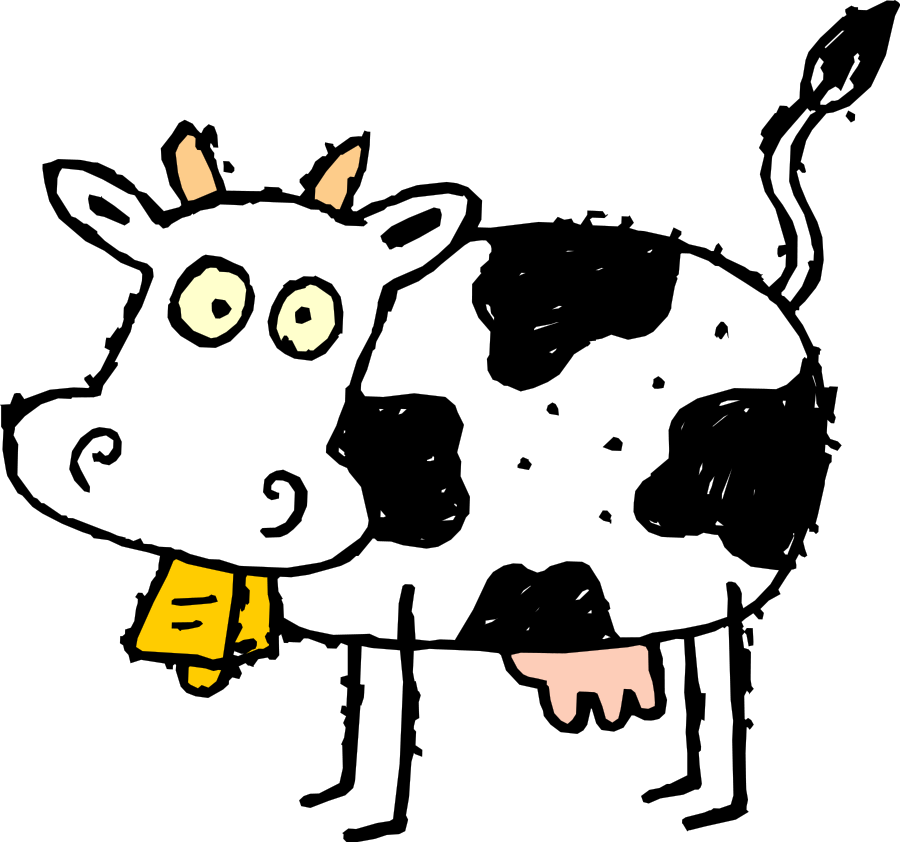
\includegraphics[width=.5\textwidth]{../FIGS/BiarB98i8.png}};
                \draw[->, ultra thick] (-4,0) to (cow);
                \draw[->, ultra thick, dotted] (cow) to (4,0);
                \draw[->, ultra thick, dashed] (-1,1.5) to (-1.5,2.5);
                \draw[->, ultra thick, dashed] (0,1.5) to (0,2.5);
                \draw[->, ultra thick, dashed] (1,1.5) to (1.5,2.5);
                \draw[->, ultra thick, dotted] (1,-2) to (1,-3);
            \end{tikzpicture}
    \end{center}
\end{frame}


%%%%%%%%%%%%%%%%%%%
\maxFrameImage{../FIGS/Volpe_etal-mammary-gland-metabolism-cows-cover.png}
\note{Figuring out this metabolism can help understand how to increase milk production}
\maxFrameImage{../FIGS/Volpe_etal-mammary-gland-metabolism-cows-abbreviations.png}
\note{These abbreviations are used in the diagram on the following page}
\maxFrameImage{../FIGS/Volpe_etal-mammary-gland-metabolism-cows-model-structure.png}
\note{We would not call this a steady state diagram but rather a flow diagram or, perhaps more appropriately, an interaction diagram}
\maxFrameImage{../FIGS/Volpe_etal-mammary-gland-metabolism-cows-notation.png}
\note{These are used in the equations}
\maxFrameImage{../FIGS/Volpe_etal-mammary-gland-metabolism-cows-some-parameters.png}
\maxFrameImage{../FIGS/Volpe_etal-mammary-gland-metabolism-cows-model1.png}
\maxFrameImage{../FIGS/Volpe_etal-mammary-gland-metabolism-cows-model2.png}
\maxFrameImage{../FIGS/Volpe_etal-mammary-gland-metabolism-cows-model3.png}


%%%%%%%%%%%%%%%%%%%
\maxFrameImage{../FIGS/Wang_etal-cows-methane-emissions-cover.png}
\note{Important in particular because of concerns about climate change. Methane makes up 16\% of the anthropogenic greenhouse gas emissions, of which 40\% comes from agriculture.}
\maxFrameImage{../FIGS/Wang_etal-cows-methane-emissions-model1.png}
\maxFrameImage{../FIGS/Wang_etal-cows-methane-emissions-model2.png}
\maxFrameImage{../FIGS/Wang_etal-cows-methane-emissions-variables-params.png}
\maxFrameImage{../FIGS/Wang_etal-cows-methane-emissions-experimental1.png}
\maxFrameImage{../FIGS/Wang_etal-cows-methane-emissions-experimental2.png}
\maxFrameImage{../FIGS/Wang_etal-cows-methane-emissions-experimental3.png}
\maxFrameImage{../FIGS/Wang_etal-cows-methane-emissions-experimental4.png}
\maxFrameImage{../FIGS/Wang_etal-cows-methane-emissions-data.png}
\maxFrameImage{../FIGS/Wang_etal-cows-methane-emissions-variables.png}
\maxFrameImage{../FIGS/Wang_etal-cows-methane-emissions-sims_vs_data.png}
\note{Colour is morning and afternoon. Important is third figure, which shows the match between predicted and observed values}


%%%%%%%%%%%%%%%%%%%
\maxFrameImage{../FIGS/Appuhamy_etal-manure-lactating-cows-cover.png}
\note{Another byproduct of cattle husbandry: manure}
\maxFrameImage{../FIGS/Appuhamy_etal-manure-lactating-cows-model.png}
\note{This is a statistical model, the only one in this course}
\maxFrameImage{../FIGS/Appuhamy_etal-manure-lactating-cows-equations.png}
\maxFrameImage{../FIGS/Appuhamy_etal-manure-lactating-cows-statistics.png}


%%%%%%%%%%%%%%%%%%%
%%%%%%%%%%%%%%%%%%%
\subsection{Models for herds}
\note{So far, we have seen models of the production of milk as well as two byproducts of cattle husbandry: methane and manure. We come back to manure later (how to get rid of it) and see how growth of weight can be modelled when we look at other animals. 

For now, let's look at herds}

\begin{frame}{At the herd level}
    \begin{center}
        \begin{tikzpicture}
            \node[inner sep=0pt] (cow1) at (0,0)
                {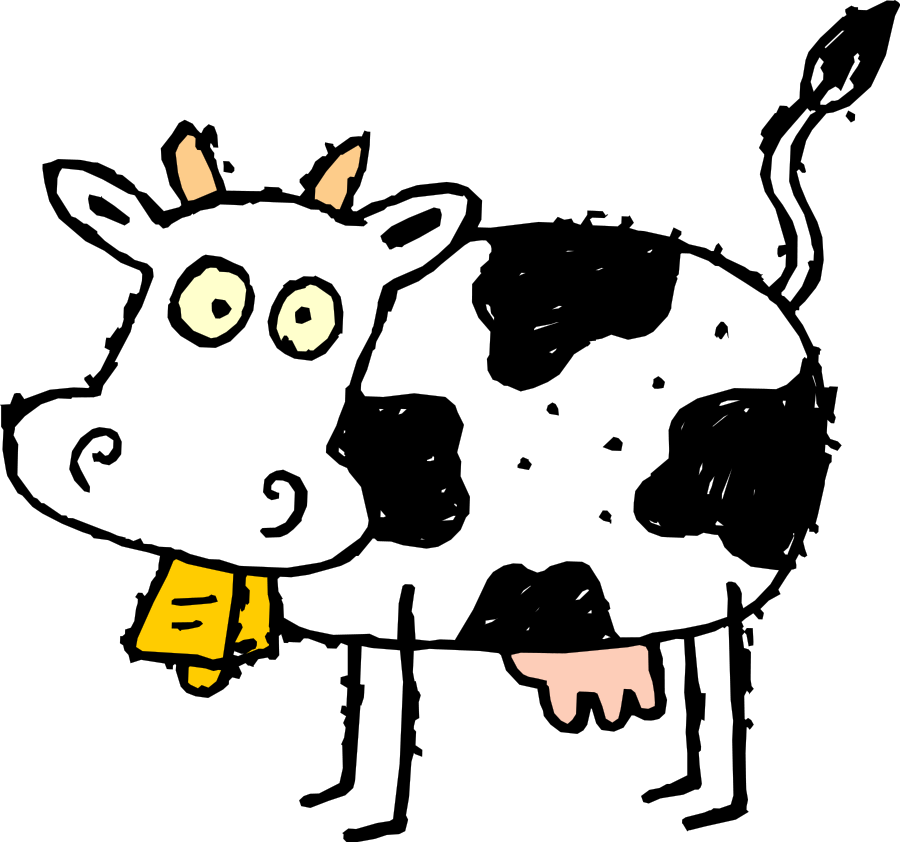
\includegraphics[width=.3\textwidth]{../FIGS/BiarB98i8.png}};
                \node[inner sep=0pt] (cow2) at (2,0)
                {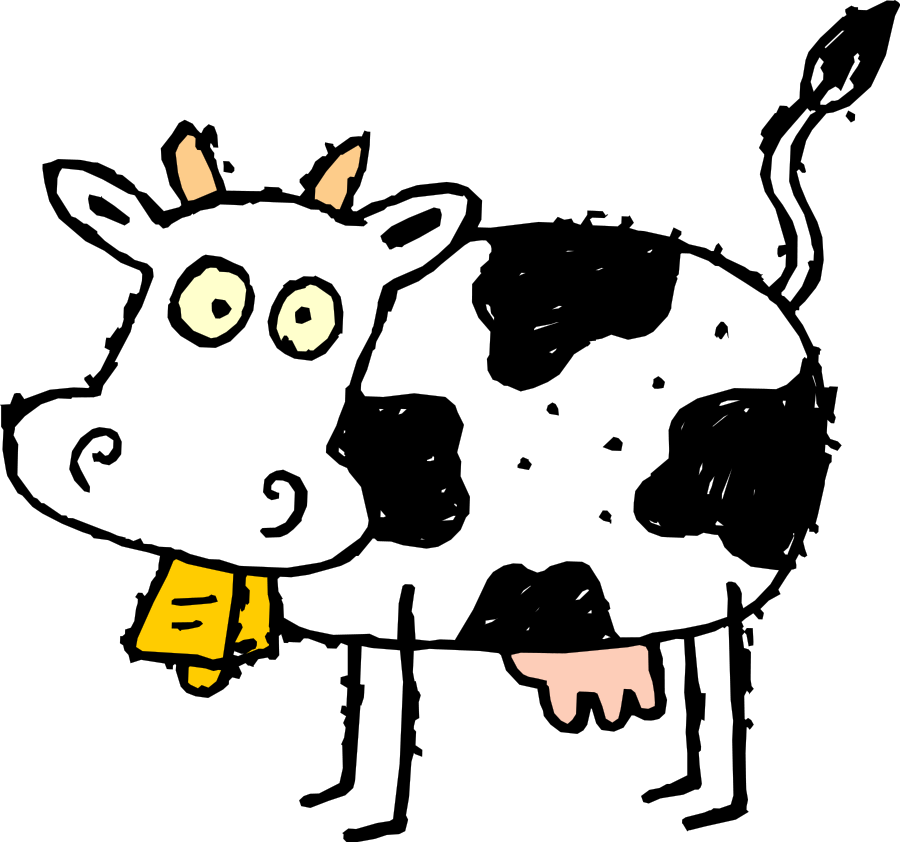
\includegraphics[width=.3\textwidth]{../FIGS/BiarB98i8.png}};
                \node[inner sep=0pt] (cow3) at (1,2)
                {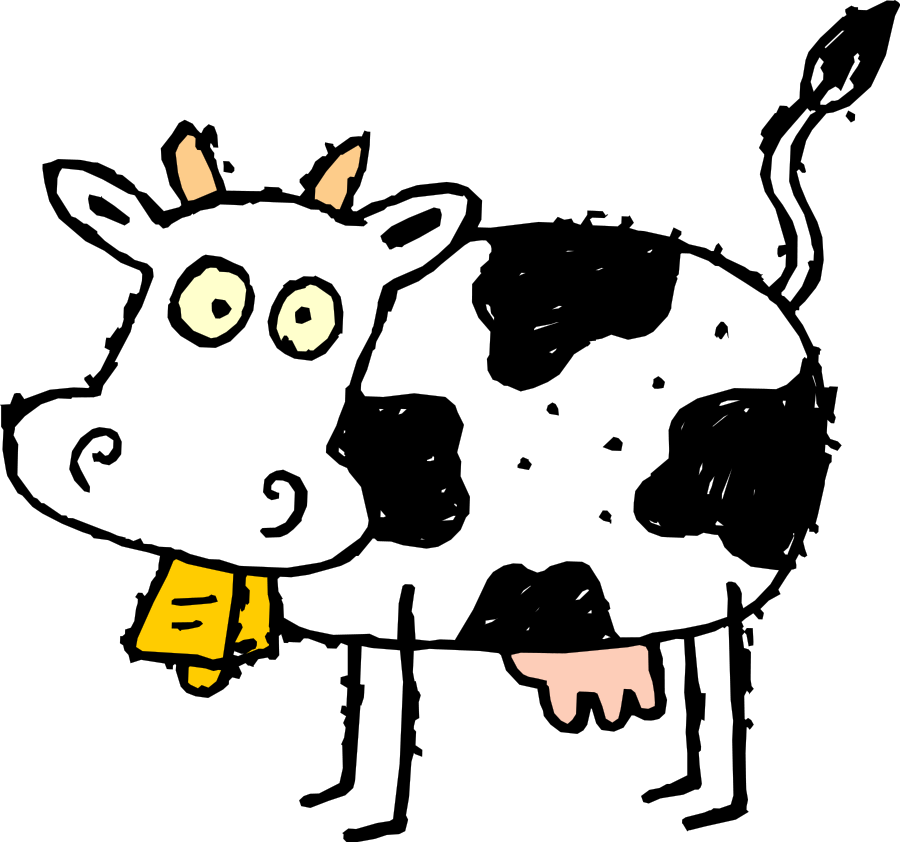
\includegraphics[width=.3\textwidth]{../FIGS/BiarB98i8.png}};
                \node[inner sep=0pt] (cow4) at (0.5,-1.5)
                {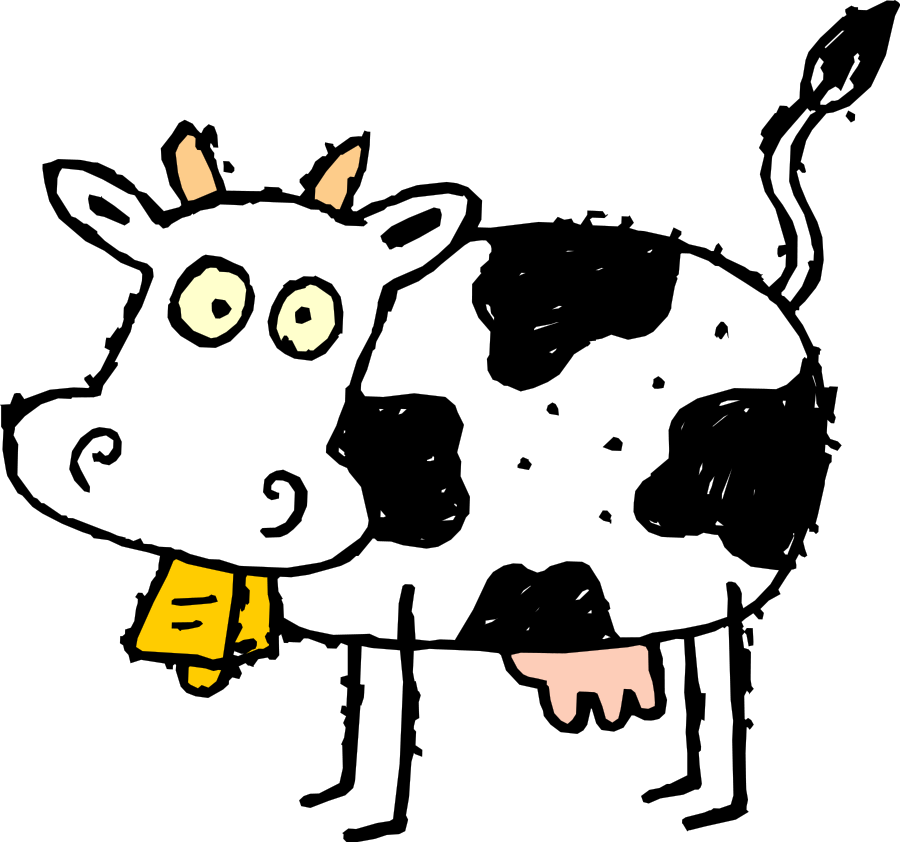
\includegraphics[width=.3\textwidth]{../FIGS/BiarB98i8.png}};
                \node[inner sep=0pt] (cow5) at (2.5,1.5)
                {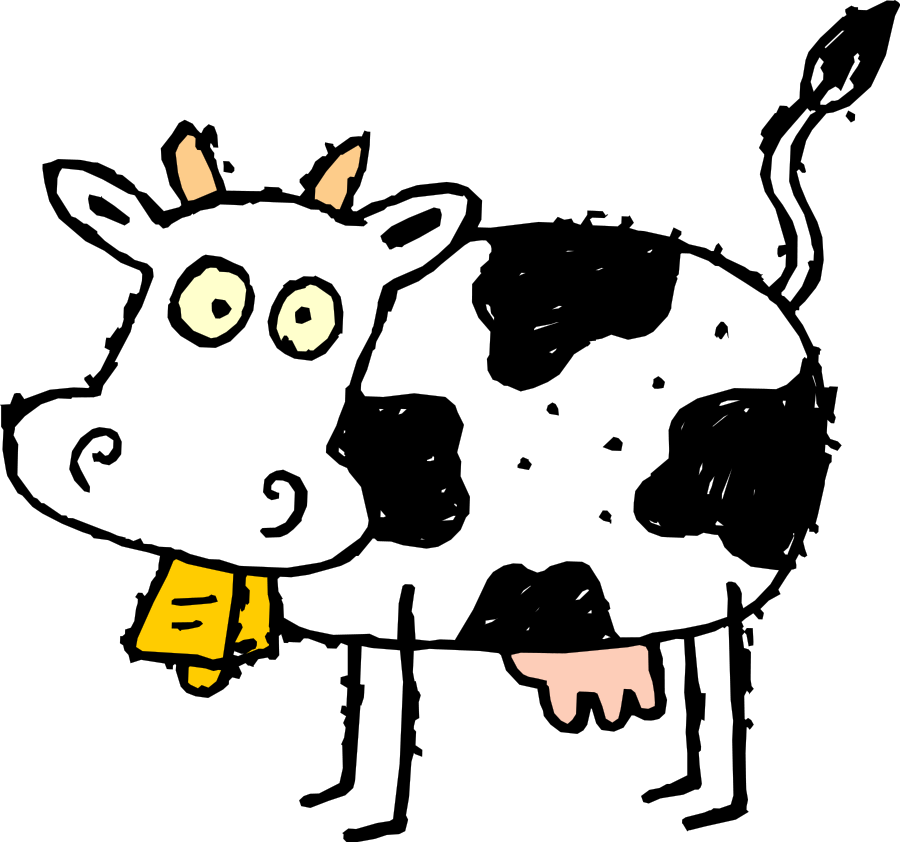
\includegraphics[width=.3\textwidth]{../FIGS/BiarB98i8.png}};
        \end{tikzpicture}
    \end{center}
\end{frame}


%%%%%%%%%%%%%%%%%%%
\maxFrameImage{../FIGS/Sun_etal-cow-sync-cover.png}
\note{Very interesting, albeit quite abstract, model.

Uses so-called switching systems

Very cool model}
\maxFrameImage{../FIGS/Sun_etal-cow-sync-single-cow-model.png}
\note{Start with a single cow

$x$ desire to eat, $y$ desire to lie down, both in $[0,1]$

Explain the model}
\maxFrameImage{../FIGS/Sun_etal-cow-sync-switching-conditions.png}
\note{$x$ desire to eat, $y$ desire to lie down, both in $[0,1]$

$\E$ eating, $\R$ resting, $\S$ standing}
\maxFrameImage{../FIGS/Sun_etal-cow-sync-switching-scenarios.png}
\note{Explain right figure first, where the squares have sides $x$ and $y$ in $[0,1]$ or $[]\delta,1]$}
\maxFrameImage{../FIGS/Sun_etal-cow-sync-coupling.png}
\maxFrameImage{../FIGS/Sun_etal-cow-sync-behaviour-coupled.png}


%%%%%%%%%%%%%%%%%%%
\maxFrameImage{../FIGS/ShiyomiTsuiki-grazing-cover.png}
\maxFrameImage{../FIGS/ShiyomiTsuiki-grazing-explain.png}
\maxFrameImage{../FIGS/ShiyomiTsuiki-grazing-model1.png}
\maxFrameImage{../FIGS/ShiyomiTsuiki-grazing-model2.png}
\maxFrameImage{../FIGS/ShiyomiTsuiki-grazing-model3.png}
\maxFrameImage{../FIGS/ShiyomiTsuiki-grazing-model4.png}
\maxFrameImage{../FIGS/ShiyomiTsuiki-grazing-model5.png}
\maxFrameImage{../FIGS/ShiyomiTsuiki-grazing-model6.png}
\maxFrameImage{../FIGS/ShiyomiTsuiki-grazing-model7.png}
\maxFrameImage{../FIGS/ShiyomiTsuiki-grazing-troop-length-theory.png}
\maxFrameImage{../FIGS/ShiyomiTsuiki-grazing-experiments.png}
\maxFrameImage{../FIGS/ShiyomiTsuiki-grazing-experimental-data.png}
\maxFrameImage{../FIGS/ShiyomiTsuiki-grazing-fitted-troop-lengths.png}


%%%%%%%%%%%%%%%%%%%
\maxFrameImage{../FIGS/Coleman_etal-plant-animal-interface-cover.png}
\maxFrameImage{../FIGS/Coleman_etal-plant-animal-interface-animals-plants.png}
\maxFrameImage{../FIGS/Coleman_etal-plant-animal-interface-diet-selection.png}


%%%%%%%%%%%%%%%%%%%
\maxFrameImage{../FIGS/Gregorini_etal-grazing-cover.png}
\maxFrameImage{../FIGS/Gregorini_etal-grazing-model1.png}
\maxFrameImage{../FIGS/Gregorini_etal-grazing-model2.png}
\maxFrameImage{../FIGS/Gregorini_etal-grazing-model3.png}
\maxFrameImage{../FIGS/Gregorini_etal-grazing-sim.png}
\maxFrameImage{../FIGS/Gregorini_etal-grazing-parameters1.png}
\maxFrameImage{../FIGS/Gregorini_etal-grazing-parameters2.png}


%%%%%%%%%%%%%%%%%%%
\maxFrameImage{../FIGS/Keshtkar_etal-reactor-manure-cover.png}
\maxFrameImage{../FIGS/Keshtkar_etal-reactor-manure-reactor-structure.png}
\maxFrameImage{../FIGS/Keshtkar_etal-reactor-manure-kinetics.png}
\maxFrameImage{../FIGS/Keshtkar_etal-reactor-manure-nomenclature.png}
\maxFrameImage{../FIGS/Keshtkar_etal-reactor-manure-chemistry.png}
\maxFrameImage{../FIGS/Keshtkar_etal-reactor-manure-equations1.png}
\maxFrameImage{../FIGS/Keshtkar_etal-reactor-manure-equations2.png}
\maxFrameImage{../FIGS/Keshtkar_etal-reactor-manure-sim.png}


%%%%%%%%%%%%%%%%%%%
%%%%%%%%%%%%%%%%%%%
%%%%%%%%%%%%%%%%%%%
%%%%%%%%%%%%%%%%%%%
\section{Models for other herds}


%%%%%%%%%%%%%%%%%%%
\maxFrameImage{../FIGS/Pla-sow-herds-cover.png}
\maxFrameImage{../FIGS/Pla-sow-herds-events.png}
\maxFrameImage{../FIGS/Pla-sow-herds-models-reviewed.png}

%%%%%%%%%%%%%%%%%%%
\maxFrameImage{../FIGS/Teleken_etal-growth-models-cover.png}
\maxFrameImage{../FIGS/Teleken_etal-growth-models-models.png}
\maxFrameImage{../FIGS/Teleken_etal-growth-models-inflection-point.png}
\maxFrameImage{../FIGS/Teleken_etal-growth-models-data-used.png}
\maxFrameImage{../FIGS/Teleken_etal-growth-models-some-fits-1.png}
\maxFrameImage{../FIGS/Teleken_etal-growth-models-goodness-fit.png}
\maxFrameImage{../FIGS/Teleken_etal-growth-models-some-fits-2.png}


%%%%%%%%%%%%%%%%%%%
\maxFrameImage{../FIGS/Akinsola_etal-growth-chicken-cover.png}
\maxFrameImage{../FIGS/Akinsola_etal-growth-chicken-growth-functions.png}
\maxFrameImage{../FIGS/Akinsola_etal-growth-chicken-experimental-site.png}
\maxFrameImage{../FIGS/Akinsola_etal-growth-chicken-experimental-site2.png}
\maxFrameImage{../FIGS/Akinsola_etal-growth-chicken-estimates.png}



\begin{frame}{Heterogeneous herds}
    \begin{center}
        \begin{tikzpicture}
            \node[inner sep=0pt] (goat1) at (-1,-1.5)
                {
\includegraphics[width=.15\textwidth]{../FIGS/goat1.png}};
            \node[inner sep=0pt] (goat2) at (-0.75,1.5)
                {
\includegraphics[width=.15\textwidth]{../FIGS/goat1.png}};
            \node[inner sep=0pt] (goat3) at (4,0)
                {
\includegraphics[width=.15\textwidth]{../FIGS/goat1.png}};
                    \node[inner sep=0pt] (cow1) at (0,0)
                {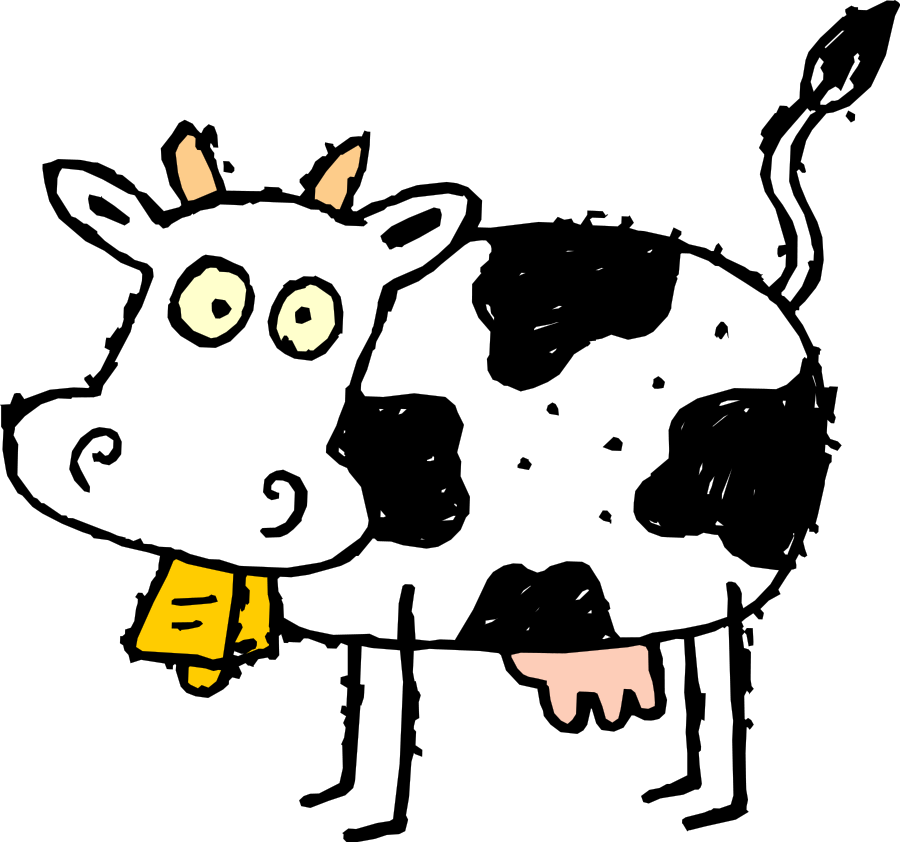
\includegraphics[width=.3\textwidth]{../FIGS/BiarB98i8.png}};
            \node[inner sep=0pt] (cow2) at (2,0)
                {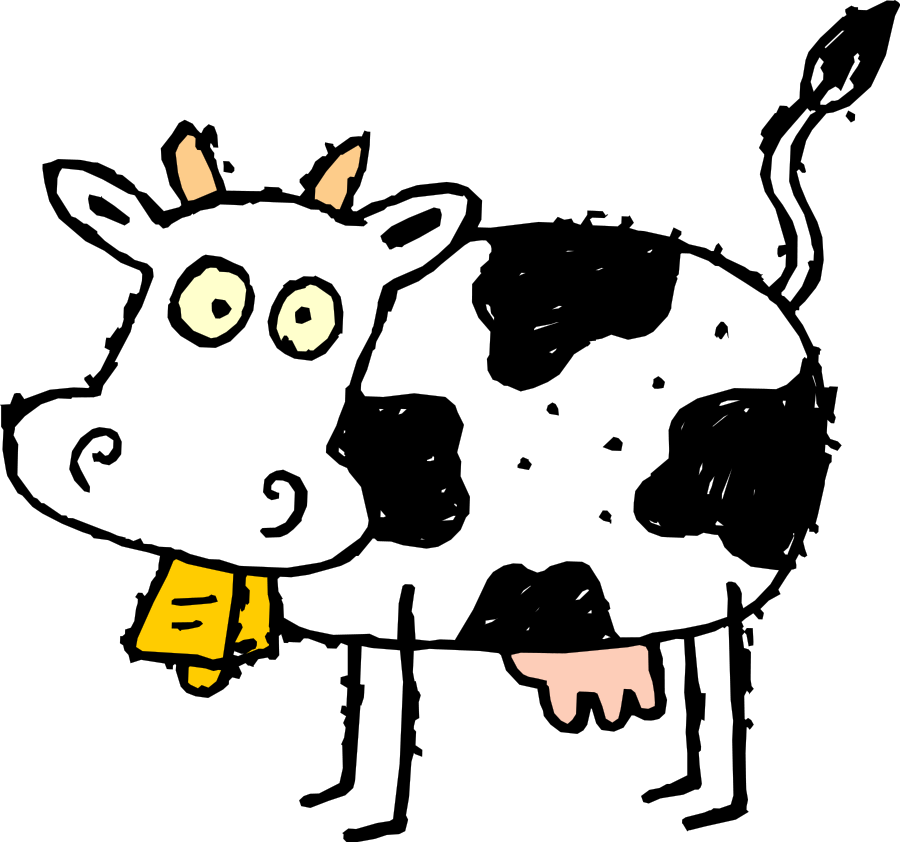
\includegraphics[width=.3\textwidth]{../FIGS/BiarB98i8.png}};
            \node[inner sep=0pt] (cow3) at (1,2)
                {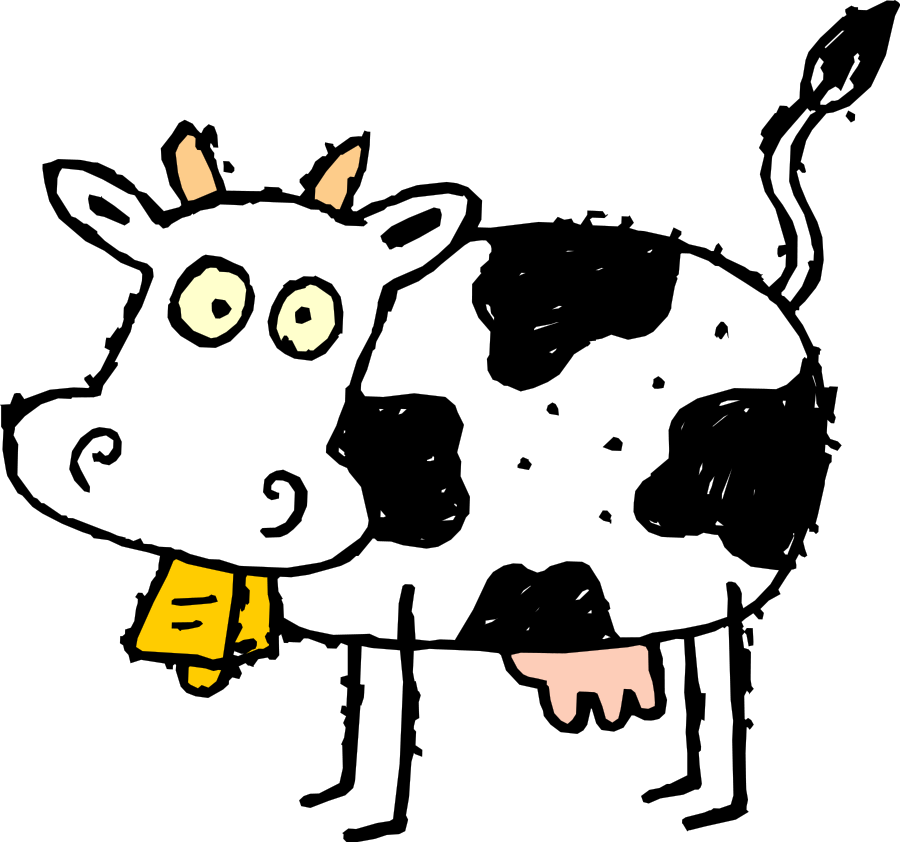
\includegraphics[width=.3\textwidth]{../FIGS/BiarB98i8.png}};
            \node[inner sep=0pt] (cow4) at (0.5,-1.5)
                {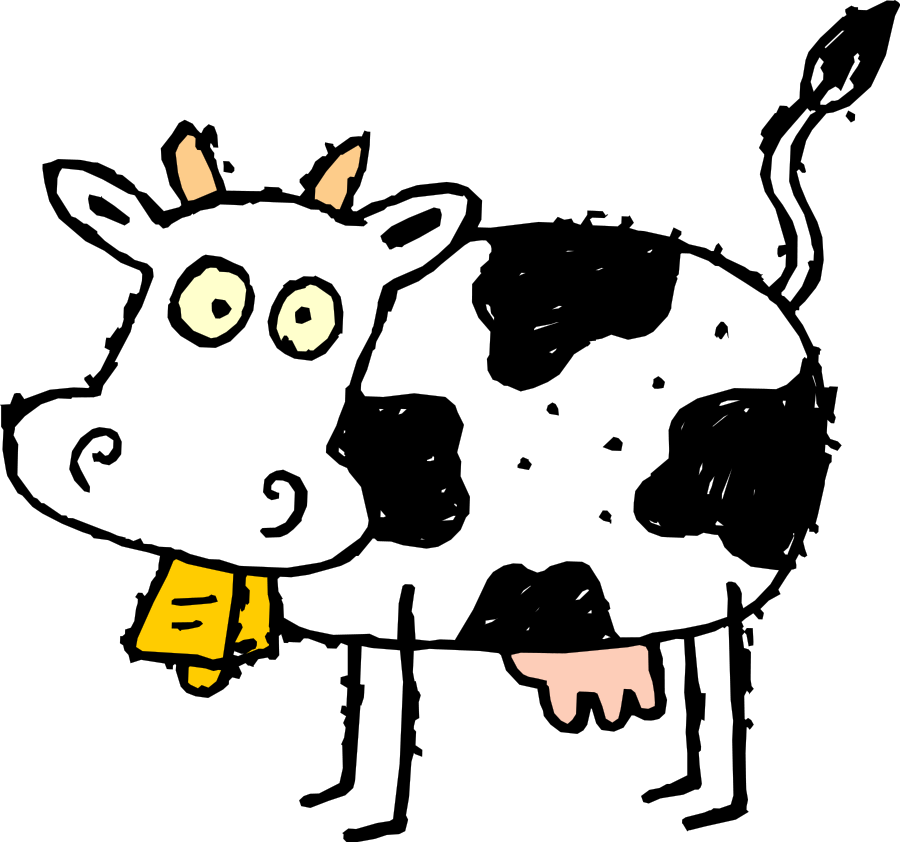
\includegraphics[width=.3\textwidth]{../FIGS/BiarB98i8.png}};
            \node[inner sep=0pt] (cow5) at (2.5,1.5)
                {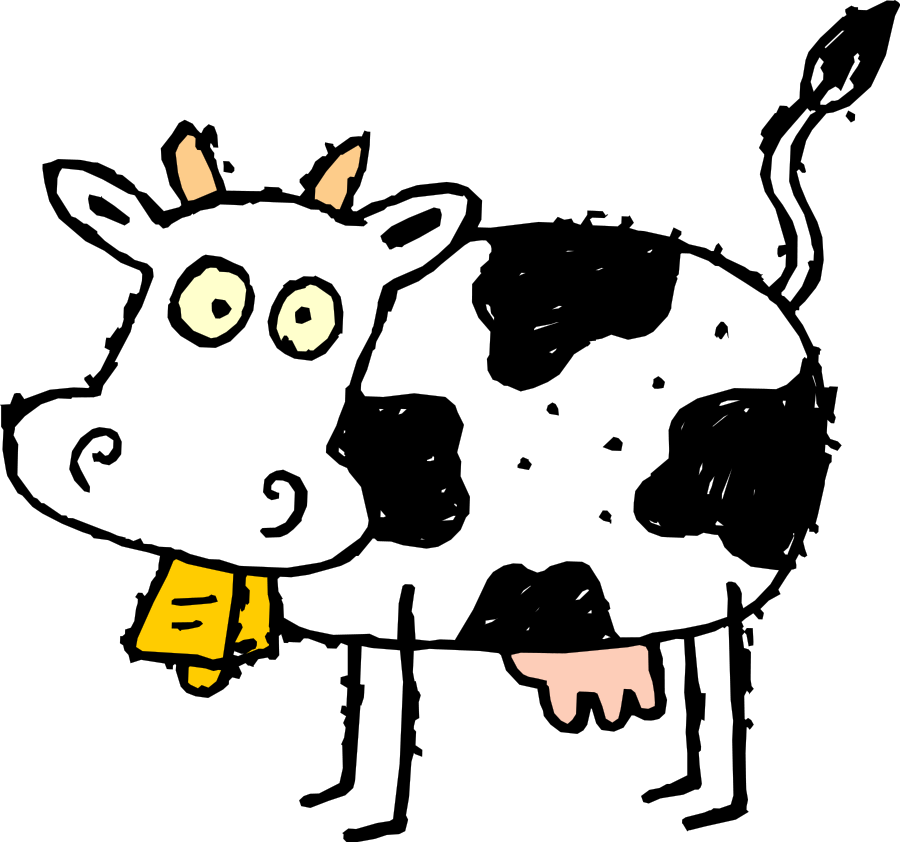
\includegraphics[width=.3\textwidth]{../FIGS/BiarB98i8.png}};
            \node[inner sep=0pt] (pig1) at (3.5,2.5)
                {
\includegraphics[width=.15\textwidth]{../FIGS/pig1.png}};
            \node[inner sep=0pt] (pig2) at (3,-2)
                {
\includegraphics[width=.15\textwidth]{../FIGS/pig1.png}};
        \end{tikzpicture}
    \end{center}
\end{frame}

%%%%%%%%%%%%%%%%%%%
\maxFrameImage{../FIGS/Shabb_etal-Mongolian-livestock-cover.png}
\maxFrameImage{../FIGS/Shabb_etal-Mongolian-livestock-overall-dynamics.png}
\maxFrameImage{../FIGS/Shabb_etal-Mongolian-livestock-model-structure.png}
\maxFrameImage{../FIGS/Shabb_etal-Mongolian-livestock-goat-equations.png}
\maxFrameImage{../FIGS/Shabb_etal-Mongolian-livestock-parameter-types.png}
\maxFrameImage{../FIGS/Shabb_etal-Mongolian-livestock-sims.png}


%%%%%%%%%%%%%%%%%%%
%%%%%%%%%%%%%%%%%%%
%%%%%%%%%%%%%%%%%%%
%%%%%%%%%%%%%%%%%%%
\section{Models for management}


%%%%%%%%%%%%%%%%%%%
\maxFrameImage{../FIGS/Hirooka-beef-prod-systems-cover.png}


%%%%%%%%%%%%%%%%%%%
\maxFrameImage{../FIGS/StygarMakulska-beef-prod-systems-cover.png}
\maxFrameImage{../FIGS/StygarMakulska-beef-prod-systems-model-types.png}


%%%%%%%%%%%%%%%%%%%
\maxFrameImage{../FIGS/Menendez_etal-modeling-animal-nutrition-cover.png}
\maxFrameImage{../FIGS/Menendez_etal-modeling-animal-nutrition-process-with-modelling.png}
\maxFrameImage{../FIGS/Menendez_etal-modeling-animal-nutrition-conceptual.png}
\maxFrameImage{../FIGS/Menendez_etal-modeling-animal-nutrition-continuous-vs-rotational.png}
\maxFrameImage{../FIGS/Menendez_etal-modeling-animal-nutrition-precision-system-models.png}
\maxFrameImage{../FIGS/Menendez_etal-modeling-animal-nutrition-some-models.png}


%%%%%%%%%%%%%%%%%%%
%%%%%%%%%%%%%%%%%%%
%%%%%%%%%%%%%%%%%%%
%%%%%%%%%%%%%%%%%%%
\section{Conclusion}

\begin{frame}{Conclusion}
    Many interesting models
    \vfill
    (Many models have never been ``properly'' studied mathematically and are ``waiting'' for an analysis)
    \vfill
    I showed only one statistical model, but the majority of published work used to be statistical 
    \vfill
    Contrary to other fields: easy to generate data of good quality
    \vfill 
    I voluntarily excluded disease-related works.. but they are easy to find!
\end{frame}


\end{document}
